\documentclass{article}

% Language setting
% Replace `english' with e.g. `spanish' to change the document language
\usepackage[english]{babel}

% Set page size and margins
% Replace `letterpaper' with `a4paper' for UK/EU standard size
% \usepackage[letterpaper,top=2cm,bottom=2cm,left=3cm,right=3cm,marginparwidth=1.75cm]{geometry}
\usepackage[letterpaper,top=2cm,bottom=2cm,left=3cm,right=3cm]{geometry}

% Useful packages
\usepackage{amsmath,amssymb}
\usepackage{graphicx}
\usepackage[colorlinks=true, allcolors=blue]{hyperref}
\usepackage{cite}
\usepackage{caption}
\usepackage{subcaption}



%\setlength{\parindent}{0pt}

\title{%

\includegraphics[width=0.5\textwidth]{dauphine.png}~ 
\\[3cm]
Optimization Project - IASD 2022-23 \\ }

\author{Maximilien Wemaere}
\date{19/09/2022-15/01/2023}

\begin{document}

\maketitle

\tableofcontents

\newpage

\section*{Introduction}

This project aims to implement the different algorithms seen in the optimization syllabus of the M2-IASD program. All the codes are available at: \path{https://github.com/MxWmr/optimization_project.git} \\ 

Please note that this report is only a complement of the different notebooks which constitute the main part of the work

\section{Gradient Descent}

\subsection{Dataset presentation}
    The data used is from the dataset \textit{Life Expectancy} which contain different factors influencing life expectancy and is provided by the World Health Organization. The aim is to predict the life expectancy (LE) of a country with the different factors of it. \\
    
    There is 22 column, and we delete 3 of them because they will not help to determine the LE ('country','year,''status') plus the LE column. So there is 18 dimensions to our optimization problem. \\

    We have 2938 points in our dataset, but if we drop all rows with a a NA value, we have only 1649 points. So we use a training set of 1349 points and a test set of 300 points. \\

    The model chosen is a linear regression, so we have an optimization problem with 18 parameters. \\

    Before we start, we normalize our data by setting the mean to 0 and the standard deviation to 1. \\

    Then we print our correlation matrix: 

    \begin{figure}[!h]
    \centering
    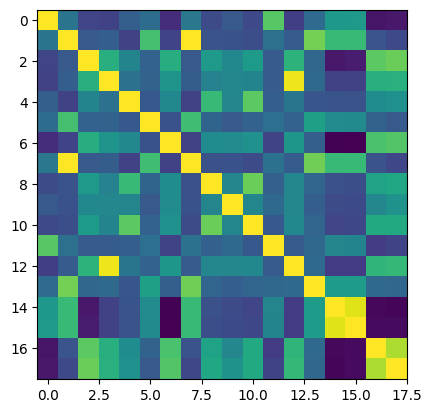
\includegraphics[width=0.5\textwidth]{images/corr.png}
    \caption{Correlation Matrix}
    \label{fig:res}
    \end{figure}

    \newpage

    We can see some high correlation between columns, such as Infant deaths and under-five death or percentage expenditure and GDP (which is pretty logic).

\subsection{Gradient descent}
    We implement gradient descent, and we test it with a learning rate of $1/||A||_{2}^2$ which is theoretically optimal, the value here is: $1.27e-4$. We add a small ridge penalty with a coefficient of $2.3e-3$. The algorithm stop when the gradient is close enough to 0. Here it ends with a test loss of $6.9$ after 9 iterations (epochs).

    \begin{figure}[!h]
    \centering
    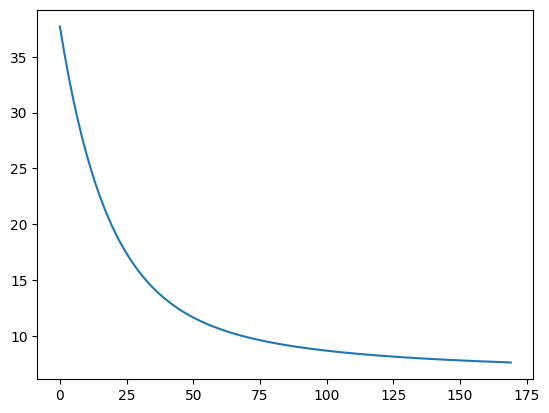
\includegraphics[width=0.6\textwidth]{images/loss1.png}
    \caption{loss evolution with GD}
    \label{fig:loss1}
    \end{figure}

    Then we vary the learning rate (or step-size) around the theoretical optimal step and we print the evolution of the loss:

     \begin{figure}[!h]
    \centering
    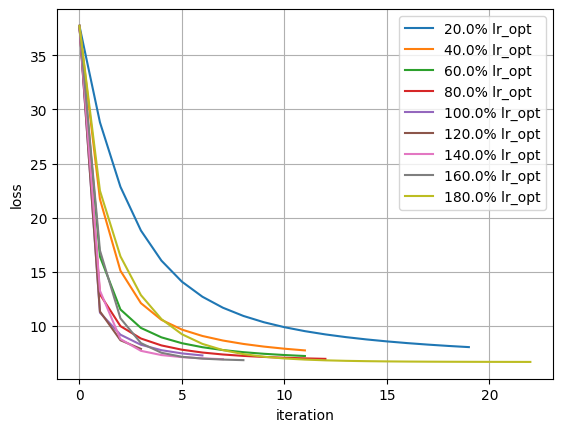
\includegraphics[width=0.6\textwidth]{images/loss2.png}
    \caption{loss evolution with different step-sizes}
    \label{fig:loss2}
    \end{figure}   

    As we expected the best learning rate is more or less the theoretical one which stop here the first, after a dozen of iterations.
\\
    If we plot the loss of the test set according to the step size:
\newpage
    \begin{figure}[!h]
    \centering
    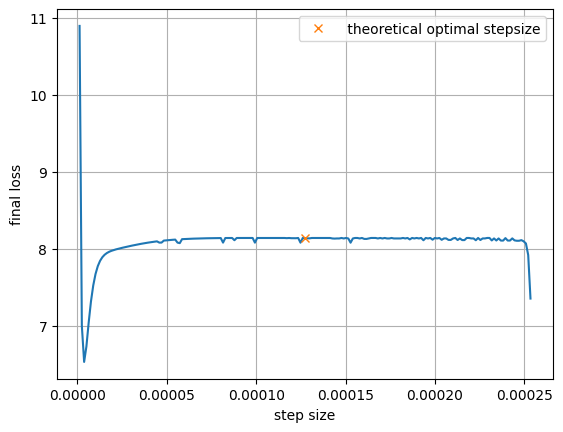
\includegraphics[width=0.6\textwidth]{images/part1.png}
    \caption{}
    \label{fig:part1}
    \end{figure}   
    

    Finally we vary the coefficient of the ridge penalty. 
    
     \begin{figure}[!h]
    \centering
    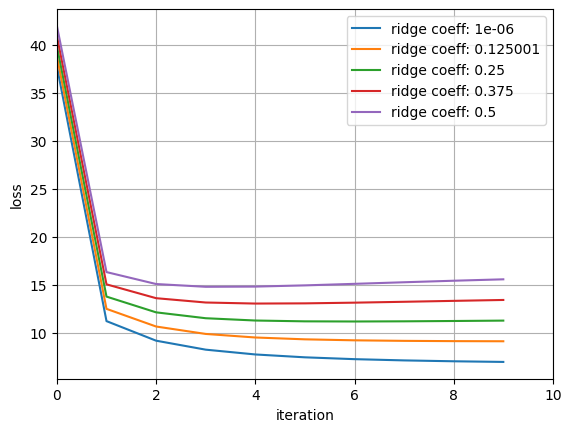
\includegraphics[width=0.6\textwidth]{images/loss3.png}
    \caption{loss evolution with different ridge penalties}
    \label{fig:loss3}
    \end{figure}   

    Here the best ridge coefficient is 0.05, if we use a higher coefficient, the algorithm do not converge and if we use a smaller the algorithm converge more slowly. So for each optimization problem we have to find this equilibrium: the largest coefficient of ridge penalty such as the algorithm converges


    
\section{Automatic differentiation}

    In this section, we were asked to implement a full backpropagation algorithm from scratch, using only numpy. \\

    After all requested elements have been coded we obtain a multilayer perceptron with the chosen number of neurons and layers, optimized by a SGD algorithm (detail of this algorithm in the next part). \\

    For the test we use two hidden layers of two and three neurons.
    For the test set: $X=[[1.,2],[2,4],[8,12],[3,5],[2,3],[4,1]]$ and $Y=[3,6,20.,8,5,5]$
    We have a good decreasing loss curve: 

    \begin{figure}[!h]
    \centering
    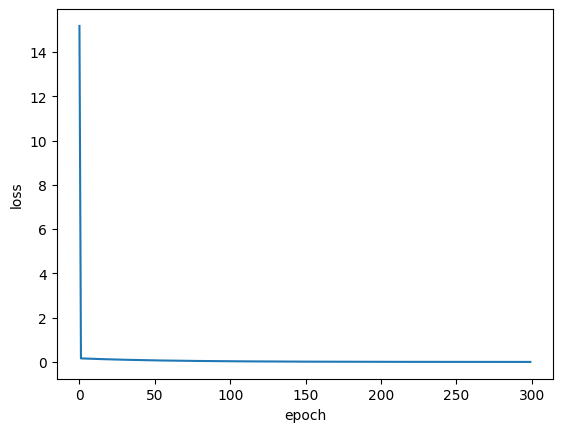
\includegraphics[width=0.6\textwidth]{images/part2.png}
    \caption{}
    \label{fig:part2}
    \end{figure}   
    
    And the results are close from the expected ones (expected results, experimental results): \\
    3.0 [3.01219679] \\
    6.0 [6.02439359] \\
    20.0 [20.00538363] \\
    8.0 [8.0135427] \\
    5.0 [5.00134591] \\
    5.0 [4.88745341] \\

    If the number of neurons or layer increase, the results tend to be less precise. For a simple problem it is not necessary to use a big perceptron.

    

\section{Stochastic Gradient}
    \subsection{SG without batch}

    First we implement the Stochastic gradient algorithm without batches. In the same setting (problem, learning rate, hyperparameters) than the gradient descent, our algorithm stop after 2600 iterations (which is equivalent to 2600/1349 = 2 epoch so 2 iteration of a GD). So SG algorithm is faster than the GD one but the test loss is $7.2$ so worse than the GD which was $6.9$. \\

    But if we change the hyperparameter $\epsilon$ which is the minimal gradient to stop the algorithm, and we diminish it we have better results: test loss of $7.2$ after 10 epochs. This confirm the theory: SG tend to converge faster than GD but is less precise.
    \begin{figure}[!h]
    \centering
    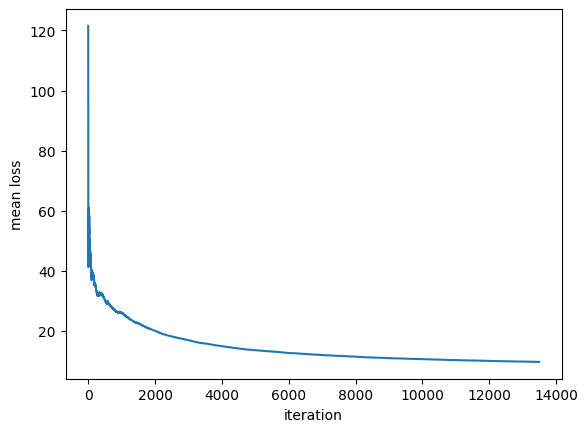
\includegraphics[width=0.6\textwidth]{images/part3_SGD.png}
    \caption{loss evolution with SG}
    \label{fig:sg1}
    \end{figure}      

    \newpage

    \subsection{Batch SG}

    Now we implement a batch size, and for different batch size we print an empirical mean of the final loss (with 30 samples) and we print it:

    \begin{figure}[!h]
    \centering
    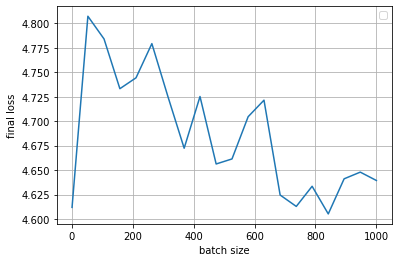
\includegraphics[width=0.6\textwidth]{images/sg2.png}
    \caption{loss evolution with different batch sizes}
    \label{fig:sg2}
    \end{figure}      

    As we can see, choose the right batch size is a complex art, and it depends of the problem.

    \subsection{SAGA method}

    We have then implemented the SAGA method to compare it with the standard SG method. This method implement different gradient which include table of specific gradients top keep in memory. With a learning rate of $0.001$ and 10 epochs, we have a test loss of $8.12$.

    \begin{figure}[!h]
    \centering
    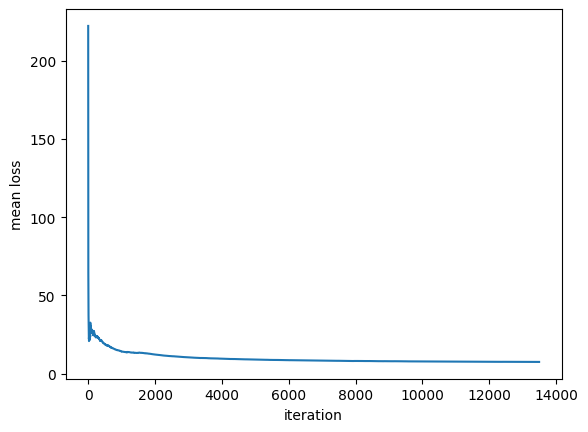
\includegraphics[width=0.6\textwidth]{images/part3_SAGA.png}
    \caption{loss evolution with SAGA method}
    \label{fig:sg3}
    \end{figure}      

    \newpage

\section{Convexity and constrained optimization}
    For this section, we implemented two algorithms which constrained the solutions of the problem to a given set. 
    
    \subsection{Conditional gradient}
        The conditional algorithm or Franck-Wolfe algorithm does not project the solution to the target set but use a trick of choosing a vector s which minimizes $\textless \nabla f , s \textgreater $ on the given set and add it to the $X$ to find. \\
        
        The difficulty of using this algorithm is to  find the good set in which we will search the solution. We identify the best set that includes the solution, to be a  ball of radius $11$. However the algorithm don't give good results on this problem. \\
        
        With a l2 ball of radius 11, we have a decreasing loss but a test loss of 2365. Same thing for the l1 ball.
        \\
        
     \begin{figure}[h!]
        \begin{subfigure}{.5\textwidth}
            \centering
            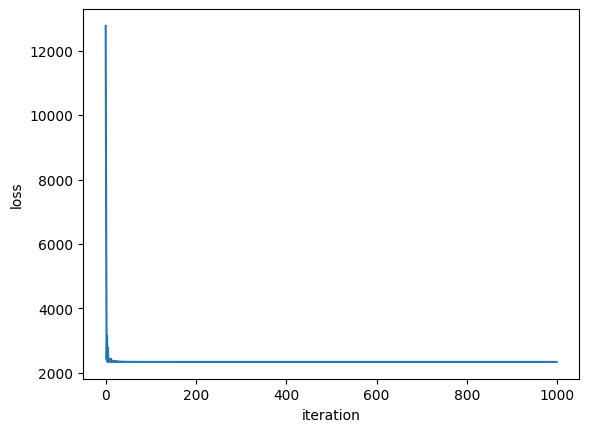
\includegraphics[width=\linewidth]{images/part4_1.png}
            \caption{Franck-Wolfe algorithm on a l2 ball}
            \label{fig:oc}
        \end{subfigure}
        \hfill
        \begin{subfigure}{.5\textwidth}
            \centering
            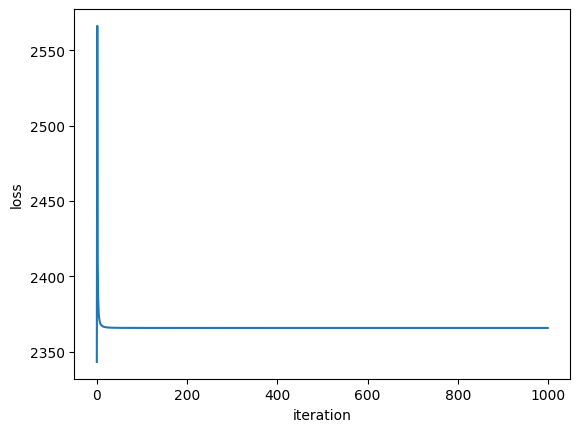
\includegraphics[width=\linewidth]{images/part4_3.png}
            \caption{Franck-Wolfe algorithm on a l1 ball}
            \label{fig:od}
        \end{subfigure}
    \end{figure}
        
        
    \subsection{Projected gradient}
        The second algorithm is the projected gradient algorithm, which is basically a gradient descent, but at each iteration we project x to the given set. \\ 
        
        Again, this algorithm don't show good results, we tested it on a l2 ball and on a simplex thanks to the method of projection on a simplex by Laurent Condat.
        
        \begin{figure}[h!]
        \begin{subfigure}{.5\textwidth}
            \centering
            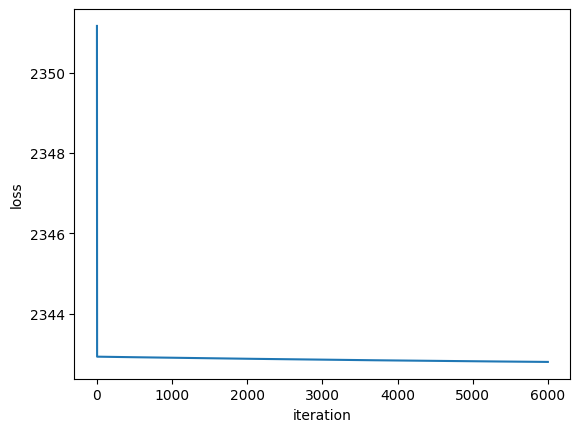
\includegraphics[width=\linewidth]{images/part4_2.png}
            \caption{Projected gradient algorithm on a l2 ball}
            \label{fig:oc}
        \end{subfigure}
        \hfill
        \begin{subfigure}{.5\textwidth}
            \centering
            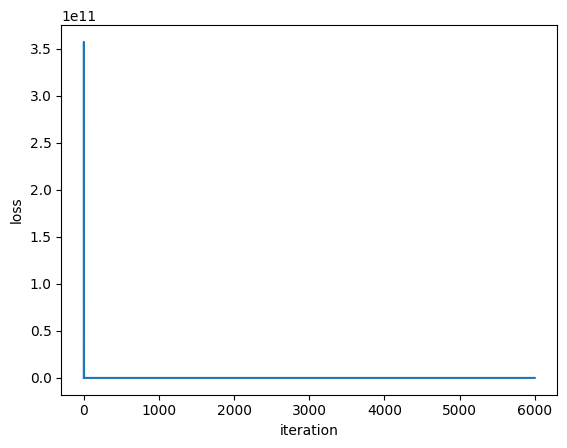
\includegraphics[width=\linewidth]{images/part4_4.png}
            \caption{Projected gradient algorithm on a simplex}
            \label{fig:od}
        \end{subfigure}
    \end{figure}     

\section{Regularization}

    In this part we implemented two different regularization: a Ridge regularization (l2) and a LASSO regularization (l1) with different regularization coefficient. All is plot on the following figure.

    \begin{figure}[!h]
    \centering
    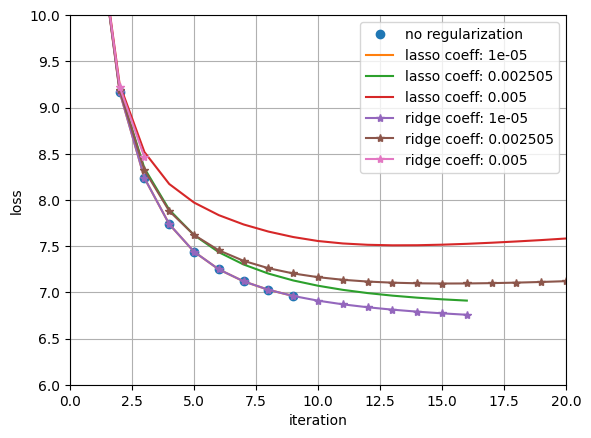
\includegraphics[width=0.6\textwidth]{images/part5.png}
    \caption{loss evolution with regularization}
    \label{fig:sg3}
    \end{figure}      

    And if we plot final loss depending on the regularization coeff, we can observe a curve that is unique to the problem. Here lasso regularization tend to be more efficient with little coefficients.

    \begin{figure}[!h]
    \centering
    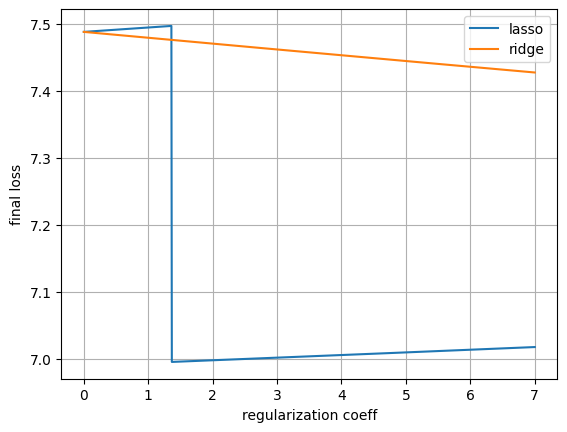
\includegraphics[width=0.6\textwidth]{images/part5_2.png}
    \caption{loss evolution with regularization}
    \label{fig:sg3}
    \end{figure}          
    

\section{Large-scale and distributed optimization}

    \subsection{Randomized block coordinate gradient descent}

        We implement an algorithm of coordinate gradient descent, with block randomized chosen blocks. After 1 epochs we have a test loss of $8.12$

    \begin{figure}[!h]
    \centering
    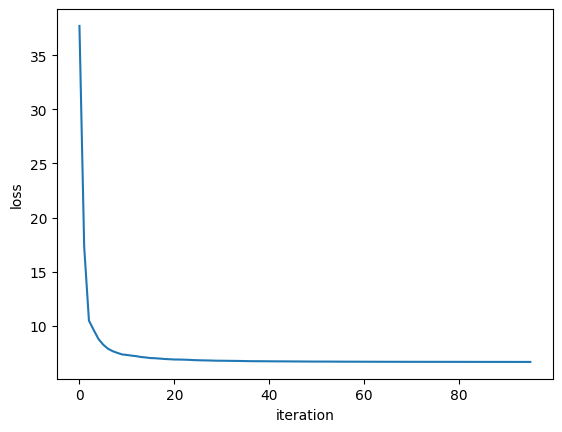
\includegraphics[width=0.6\textwidth]{images/part6_1.png}
    \caption{loss evolution with coordinate gradient}
    \label{fig:sg3}
    \end{figure}  

    And if we study the effect on block size, we can observe that a little block size is preferable.

    \begin{figure}[!h]
    \centering
    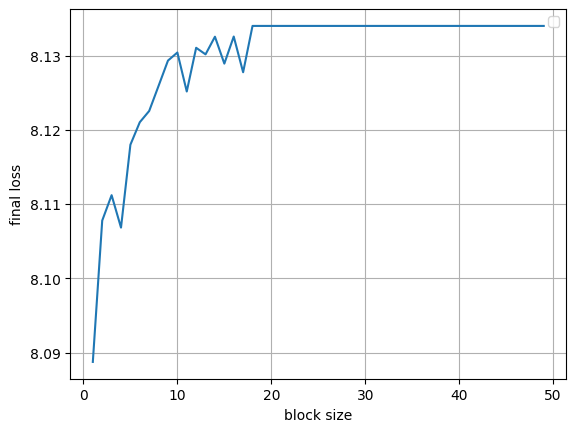
\includegraphics[width=0.6\textwidth]{images/part6_2.png}
    \caption{block size influence with coordinate gradient}
    \label{fig:sg3}
    \end{figure}  

    \newpage

    \subsection{RBCD combined with SGD}

    Then we combine the previous algorithm with SGD and we obtain a test loss of $6.7$ with 15 epochs, the algorithm is then more efficient than the simple RBCD but slower to converge.

    \begin{figure}[!h]
    \centering
    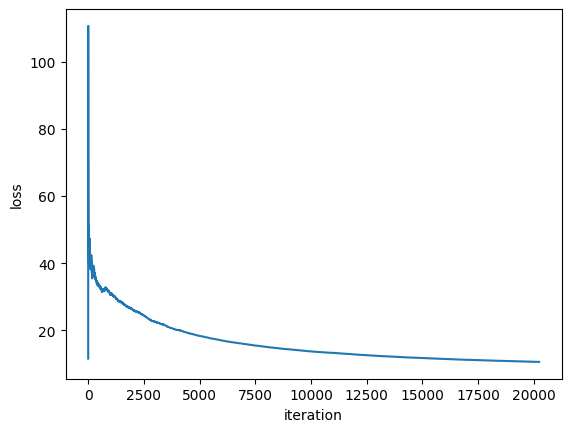
\includegraphics[width=0.6\textwidth]{images/part6_3.png}
    \caption{loss evolution with combined algorithms}
    \label{fig:sg3}
    \end{figure}  

    As we can see on the next figure, with this algorithm, the best batch size is 1

    \begin{figure}[!h]
    \centering
    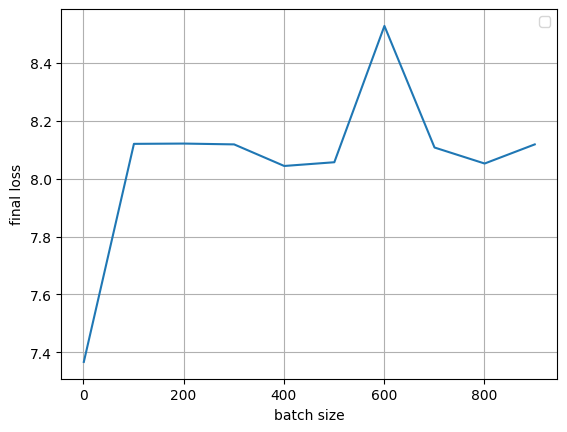
\includegraphics[width=0.6\textwidth]{images/part6_4.png}
    \caption{batch size influence with combined algorithms}
    \label{fig:sg3}
    \end{figure}  

    \newpage

\section{Advanced topics on gradient descent}

    \subsection{Heavy ball}

    We implement heavy ball on the standard gradient descent, and with a momentum coefficient (gamma) of $0.1$ we obtain a test loss of $6.5$ which is the best result until now.

    \begin{figure}[!h]
    \centering
    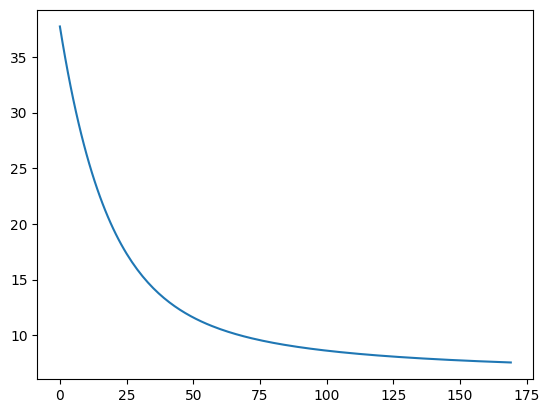
\includegraphics[width=0.6\textwidth]{images/part7_1.png}
    \caption{Gradient descent with heavy ball momentum}
    \label{fig:sg3}
    \end{figure}  

    Then, we study the influence of the momentum coefficient, and we observe that a little coefficient is preferable.

    \begin{figure}[!h]
    \centering
    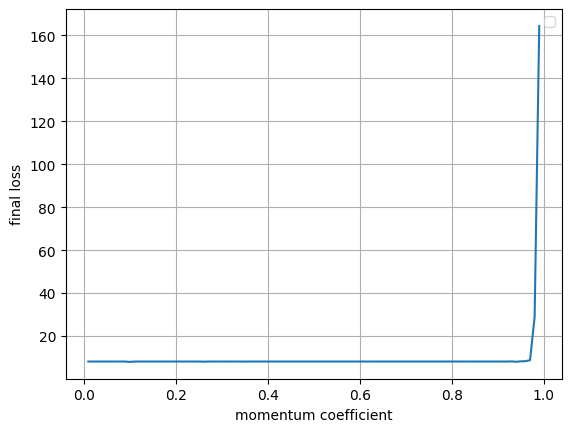
\includegraphics[width=0.6\textwidth]{images/part7_2.png}
    \caption{momentum coefficient influence}
    \label{fig:sg3}
    \end{figure}      
    
    \newpage

    We do the same study for the step size:

    \begin{figure}[!h]
    \centering
    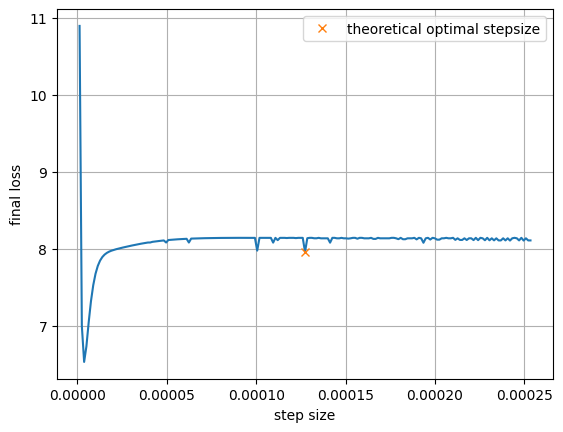
\includegraphics[width=0.6\textwidth]{images/part7_3.png}
    \caption{momentum coefficient influence}
    \label{fig:sg3}
    \end{figure}      
  
    
    \subsection{Non convex loss function}

    Here we use a non convex loss function: just à l2 loss function but with a p norm regularization and $0<p<1$. Here we use $p = 0.5$. The algorithm can't converge easily and the test loss is $29.7$. The algorithm stop before the max iteration, so it means that the gradients became very small so it means that the reach a critical point, a local minimizer.

    \begin{figure}[!h]
    \centering
    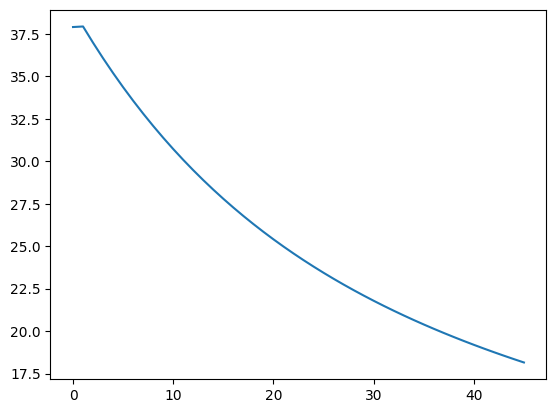
\includegraphics[width=0.6\textwidth]{images/part7_34.png}
    \caption{non convex loss evolution}
    \label{fig:sg3}
    \end{figure}       
\newpage

\section*{Conclusion}

We have reviewed different optimization methods. It turns out that with this problem, a gradient descent with regularization will often be more efficient than a more complex method. 

Only the Heavy Ball algorithm was able to obtain better results. 

However it is clear that a combination of different algorithms is often more efficient (stochastic gradient with regularization and momentum for example). This is why we are still far from the results obtained by the sklearn gradient algorithm which combines the best of all these methods.


\nocite{*}
\bibliographystyle{alpha}
\bibliography{sample}


\end{document}